\chapter{Gaussian Naive Bayes and Zero Probability}
\label{chap:gaussian_nb}

\section{Gaussian Naive Bayes (Continuous Data)}
When features are continuous (e.g., Height, Weight, Salary), we cannot "count" occurrences like in text data.
Instead, we assume that the data for each class is distributed according to a \textbf{Gaussian (Normal) Distribution}.

\subsection{The Formula}
The likelihood $P(x_i | y)$ is given by the Probability Density Function (PDF):

\begin{equation}
    P(x_i | y) = \frac{1}{\sqrt{2\pi \sigma_y^2}} \exp \left( - \frac{(x_i - \mu_y)^2}{2\sigma_y^2} \right)
\end{equation}

Where:
\begin{itemize}
    \item $\mu_y$: Mean of feature $x_i$ for class $y$.
    \item $\sigma_y^2$: Variance of feature $x_i$ for class $y$.
\end{itemize}

\textbf{Training}: Training simply involves calculating the Mean ($\mu$) and Variance ($\sigma^2$) for every feature, for every class. This makes training extremely fast.

\begin{figure}[htbp]
\centering
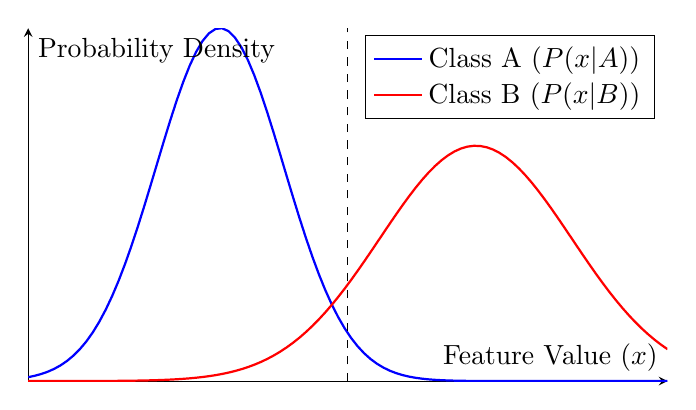
\begin{tikzpicture}
    \begin{axis}[
        xlabel={Feature Value ($x$)}, ylabel={Probability Density},
        axis lines=middle,
        width=0.8\textwidth, height=0.5\textwidth,
        ticks=none
    ]
    % Class A (Mean 3, Std 1)
    \addplot[domain=0:10, samples=100, blue, thick] {1/(sqrt(2*pi))*exp(-(x-3)^2/2)};
    \addlegendentry{Class A ($P(x|A)$)}
    
    % Class B (Mean 7, Std 1.5)
    \addplot[domain=0:10, samples=100, red, thick] {1/(sqrt(2*pi*1.5^2))*exp(-(x-7)^2/(2*1.5^2))};
    \addlegendentry{Class B ($P(x|B)$)}
    
    % New point at x=5
    \draw[dashed, black] (axis cs:5, 0) -- (axis cs:5, 0.4);
    \node at (axis cs:5, 0.42) {New Point $x=5$};
    \end{axis}
\end{tikzpicture}
\caption{Gaussian Naive Bayes. At $x=5$, the Blue curve (Class A) is higher, so $P(x|A) > P(x|B)$. We predict Class A.}
\label{fig:gaussian_nb}
\end{figure}

\section{Example: Predicting "Job Offer"}
\textbf{Feature}: CGPA.
\begin{itemize}
    \item \textbf{Class: Placed (Yes)}: Mean $\mu_{yes} = 8.5$, Std $\sigma_{yes} = 1.0$.
    \item \textbf{Class: Not Placed (No)}: Mean $\mu_{no} = 6.0$, Std $\sigma_{no} = 1.5$.
\end{itemize}

\textbf{Query}: Student with \textbf{CGPA = 7.5}.
We plug $x = 7.5$ into the Gaussian formula for both classes:
\begin{enumerate}
    \item \textbf{Likelihood (Placed)}: Evaluate Normal PDF $N(8.5, 1.0)$ at $x=7.5$.
    \item \textbf{Likelihood (Not Placed)}: Evaluate Normal PDF $N(6.0, 1.5)$ at $x=7.5$.
\end{enumerate}
Usually, the bell curve for "Placed" will give a higher density for 7.5 than "Not Placed".

\section{The Zero Frequency Problem}
\subsection{The Issue}
In Multinomial Naive Bayes (Text), we calculate likelihoods by counting words:
$$ P(\text{Word}|y) = \frac{\text{Count(Word)}}{\text{Total Words}} $$
What if a word never appears in the training data for a class?
\begin{itemize}
    \item Count = 0.
    \item Likelihood $P(\text{Word}|y) = 0$.
    \item Since we multiply all probabilities: $P \times P \times 0 = 0$.
    \item The entire Posterior becomes 0. One missing word kills the whole prediction.
\end{itemize}

\subsection{The Solution: Laplace Smoothing (Additive Smoothing)}
We add a small dummy count ($\alpha$) to every word count to ensure no probability is ever exactly zero.

\begin{equation}
    P(x_i | y) = \frac{\text{Count}(x_i) + \alpha}{\text{Total Count} + \alpha \cdot d}
\end{equation}
Where:
\begin{itemize}
    \item $\alpha$: Smoothing parameter (usually 1).
    \item $d$: Number of distinct features (Vocabulary size).
\end{itemize}

\section{HOTS: Interview Questions}
\textbf{Q1: What is "Log-Probabilities"? Why do we use them?}
\begin{itemize}
    \item Multiplying many small probabilities ($0.001 \times 0.002 \dots$) results in extremely small numbers, leading to \textbf{Numerical Underflow} (computer rounds to 0).
    \item Solution: Take the Logarithm. Multiplication becomes Addition:
    $$ \log(P(A) \cdot P(B)) = \log P(A) + \log P(B) $$
    \item Classification becomes: $\text{argmax}_y [ \log P(y) + \sum \log P(x_i | y) ]$.
\end{itemize}

\textbf{Q2: Does Gaussian Naive Bayes assume features are normally distributed?}
\begin{itemize}
    \item Yes. If your data is highly skewed or multi-modal, this assumption breaks.
    \item \textbf{Fix}: Use Power Transformation (Box-Cox or Yeo-Johnson) to make features more Gaussian before training.
\end{itemize}
